\chapter{検出器 (MAIKo TPC)}
%\section{MAIKo TPC}
\section{MAIKo TPC とは}
Time Projection Chamber (TPC) は荷電粒子のトラックを検出するために広く用いられている検出器である。
荷電粒子がMAIKo TPC のガス中を通過するときに電子を発生させる。
この電子をドリフト電場 ($y$軸方向) により読み出し面にドリフトさせることでトラックを検出する。
図\ref{fig::MAIKo_view}のようにTPC の有感領域中で入射粒子と標的粒子を反応させることで、
散乱点の周りを有感領域で覆うことができる。
そのため、散乱で放出される低エネルギーの荷電粒子を大立体角で検出することができる。
このような検出器としてMAIKo TPC が開発された。
MAIKo TPC の写真を図\ref{pic::MAIKo}に示す。
\begin{figure}
  \centering
  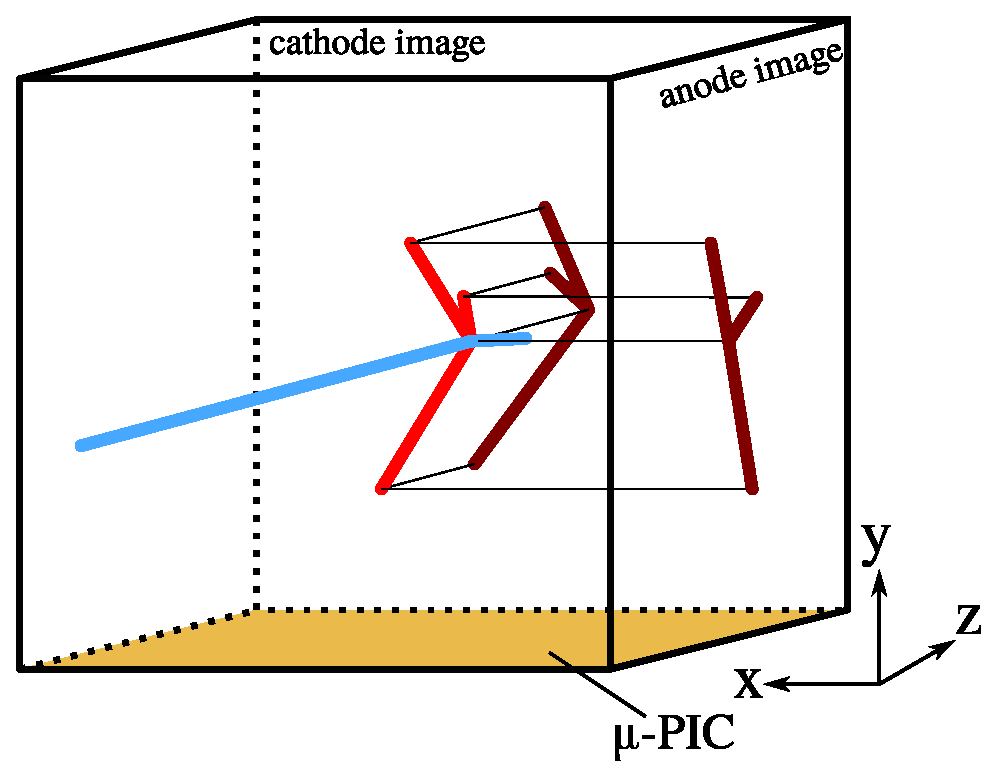
\includegraphics[clip, width=0.7\columnwidth]{eps/MAIKo2.eps}
  \caption[MAIKo TPC の概観図。]{MAIKo TPC の概観図。
    図では紙面手前から入射した中性子 (青) がTPCの中の${}^{12}{\rm C}$と散乱して3つの$\alpha$粒子 (赤) に崩壊した事象を表す。
    anode image ($zy$平面) と cathode image ($zy$平面) の2平面に荷電粒子のトラックが射影される。
    中性子は電荷を持たないためanode \& cathode image にトラックとして検出されない。
  }
  \label{fig::MAIKo_view}
\end{figure}
\begin{figure}
  \centering
%  \includegraphics[clip, width=0.7\columnwidth]{}
  \caption[MAIKo TPC の概観。]{MAIKo TPC の概観。}
  \label{pic::MAIKo}
\end{figure}
MAIKo TPC では3次元のトラックを図\ref{fig::MAIKo_view}のように2つの平面 ($zy, xy$平面) に射影された画像として取得される。

\subsection{MAIKo TPC の構造}
図\ref{fig::MAIKo_view}にMAIKo TPC の概観図、
図\ref{fig::MAIKo_cage}にMAIKo TPC の構造を示す。
\begin{figure}
  \centering
  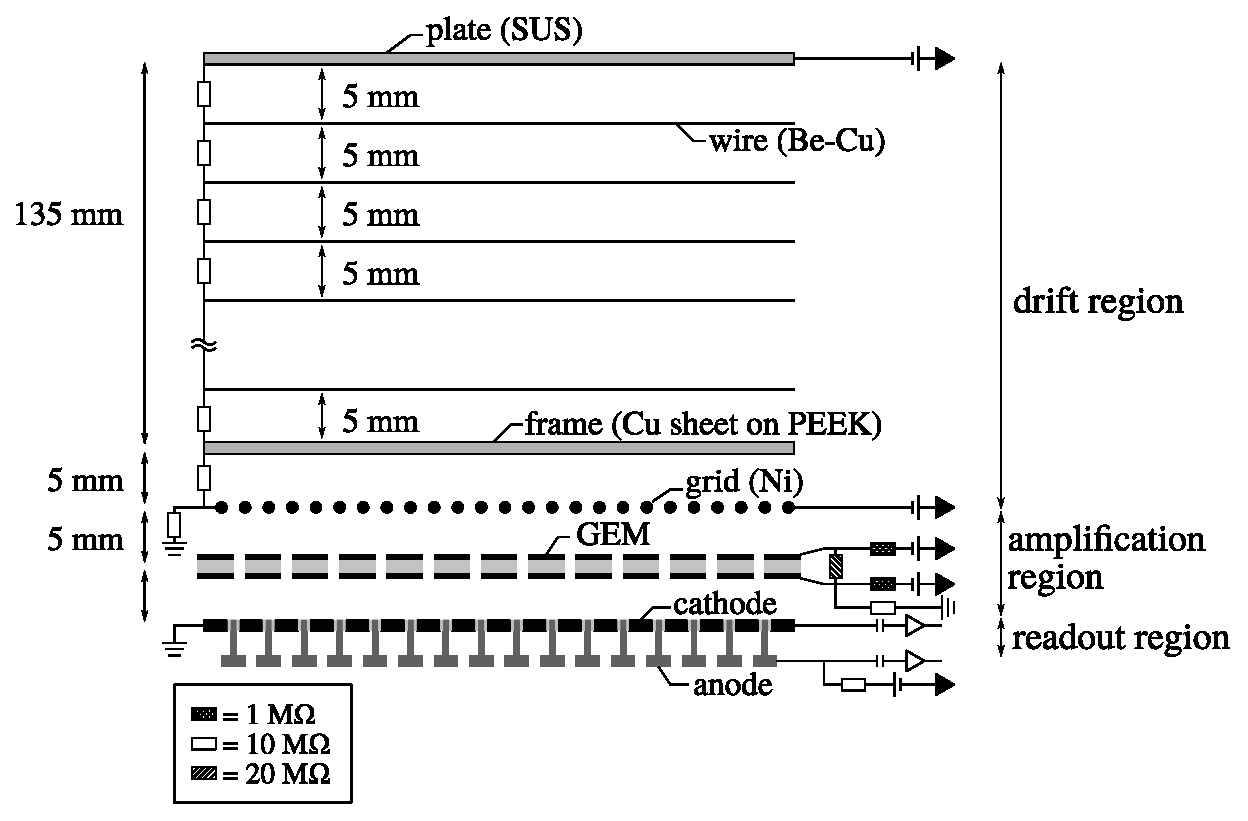
\includegraphics[clip, width=\columnwidth]{eps/MAIKo_cage.eps}
  \caption{MAIKo TPC の構造。}
  \label{fig::MAIKo_cage}
\end{figure}
plate とgrid の間のドリフト領域に電圧をかけることでドリフト電場を形成する。
ドリフト領域を荷電粒子が通過する際に生成された電子が増幅領域へ移動する。
MAIKo TPC ではGEM (gas electron multiplier) と$\mu$-PIC によってドリフト領域からドリフトしてきた電子を増幅する。
増幅した電子およびイオンによって$\mu$-PIC のanode とcathode に誘起される信号を読み出す。

\subsection{ドリフト領域}
plateとwire、grid によって囲まれた領域をドリフト領域と呼ぶ。
grid からplate の方向 (図\ref{fig::MAIKo_cage}では上向き) にドリフト電場を作ることで
荷電粒子の周りに発生した電子を増幅領域へドリフトさせる。
ドリフト電場の一様性が高いほど、電子を均等にドリフトすることができる。
ドリフト電場を一様に形成するためにwire が5 mm 間隔で巻かれている。
plate とgrid のそれぞれに高電圧をかけることによってドリフト電場を調整する。

\subsection{GEM}
$\mu$-PIC にも増幅機構があるが、より大きく増幅するためにGEM を用いた増幅機構を設けている。
GEM は、図\ref{pic::GEM}のようにポリマーのフルムの表面を銅で被覆し、
直径70 $\mu$m の穴を140 $\mu$m 間隔で1 mm$^2$あたり100 個の密度で開けたものである。
銅の2つの層はポリマーによって絶縁されている。
銅の両面に電圧を印加することによって、高電場が形成されてドリフトしてきた種電子が増幅される。
\begin{figure}
  \centering
  %\includegraphics[clip, width=0.7\colmunwidth]{}
  \caption{GEM の拡大図。}
  \label{pic::GEM}
\end{figure}

\subsection{$\mu$-PIC}
読み出しパッドである$\mu$-PICは図\ref{fig::mupic}のようにanode strip とcathode strip が垂直に配置されている。
anode strip、cathode stripともに400~$\mu$m 間隔で256~chに分割されており、
合計512~chで信号を読み出している。
\begin{figure}
  \centering
  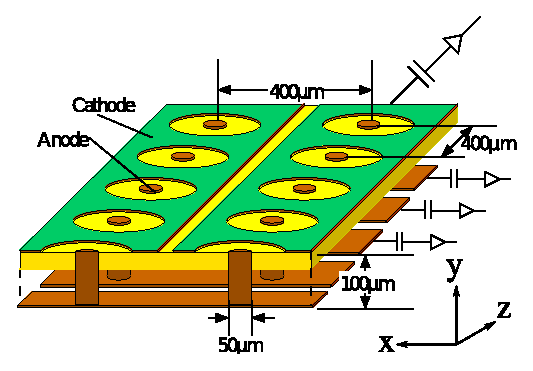
\includegraphics[clip, width=0.7\columnwidth]{eps/upic_struc_xyz.eps}
  \caption[$\mu$-PICの概観図。]{$\mu$-PICの概観図。
    図中の横方向にanode strip、奥行き方向にcathode strip が配置されている。
  }
  \label{fig::mupic}
\end{figure}
図\ref{fig::MAIKo_view}中でanode strip は$z$軸、cathode strip は$x$軸と平行に配置されている。
ドリフト電場により移動してきた電子をanode strip、cathode strip により読み出し、
それぞれ$x$軸、$z$軸座標を検出することができる。
また、anode strip、cathode strip で検出される信号の時間分布により$y$軸座標を決定することができる。

MAIKo TPC からは図\ref{fig::track_demo}のようにanode strip に垂直な面 ($z-y$平面) に射影されたトラックと
cathode strip に垂直な面 ($z-y$平面) に射影されたトラックの2つの画像が出力される。
anode strip とcathode strip はそれぞれ256~chで構成され、
読み出される信号波高の時間変化は100~MHzで1,024~samples測定される。
そのため、出力される画像の解像度は$256\times1,014$~pixels となる。
\begin{figure}
  \centering
  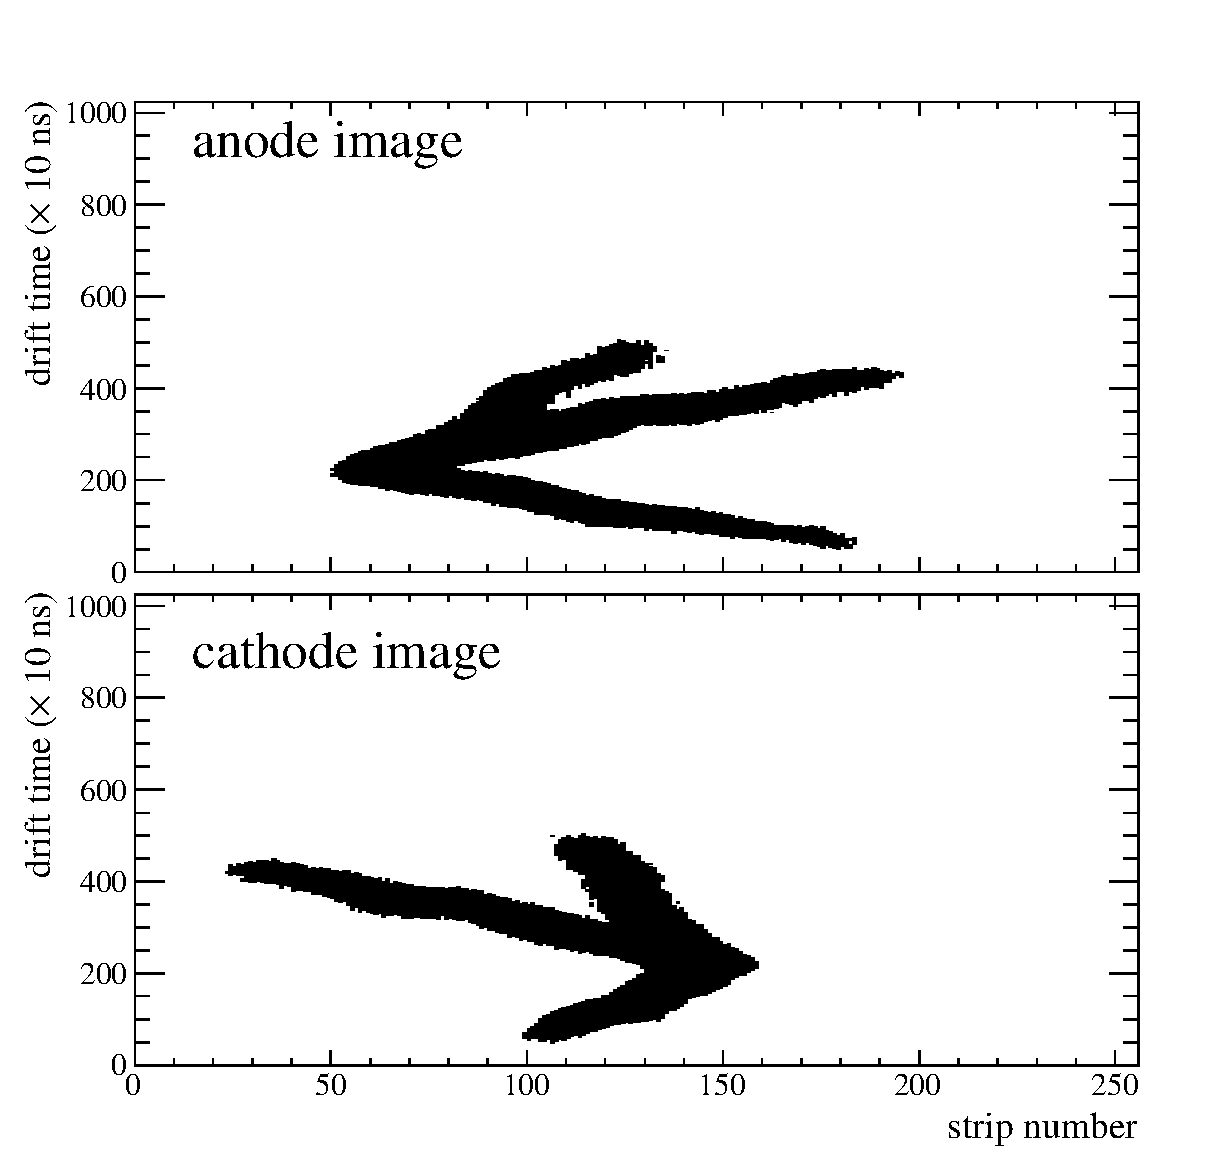
\includegraphics[clip, width=0.7\columnwidth]{eps/10016_6.eps}
  \caption[MAIKo TPC から得られず画像データの一例。]
          {MAIKo TPC から得られず画像データの一例。
          このイベントは\ref{chap::simulation}章で述べるシミュレーションによって生成したデータである。}
  \label{fig::track_demo}
\end{figure}

\section{検出ガスの候補}
標的に${}^{12}{\rm C}$を用いるため分子中に炭素を含むガスを検出ガスに用いる。
${}^{12}{\rm C}$以外の原子核が含まれるガスを用いると背景事象となるため、
水素と炭素以外の原子が含まれない炭化水素を用いる。
炭化水素には代表的なものでも、メタン (${\rm CH_{4}}$) やメタン (${\rm C_{2}H_{6}}$)、
イソブタン (iso-${\rm C_{4}H_{10}}$) などいくつもある。
また、水素ガスやヘリウムガスとの混合ガスも用いることができる。
検出ガスとして求められる性能には以下のようなものがある。
\begin{itemize}
\item
  放電しない
\item
  荷電粒子のエネルギー損失 ($dE/dx$) が適切な大きさである
\item
  ${}^{12}{\rm C}$の量が少なすぎない
\item
  適切なドリフト速度を達成できる
\item
  適切なドリフト電場のもとでディフュージョンが小さい
\end{itemize}
これらの項目を基準に検出ガスの種類と圧力の決定を行う。

\subsection{エネルギー損失}
荷電粒子のエネルギー損失 ($dE/dx$) が大きくなりすぎるとガス中での飛行距離が短くなり、
トラックとして認識することが難しくなる。
また、MAIKo TPC では粒子のエネルギーをトラックの長さから決定する。
そのため、$dE/dx$ が小さくなりすぎるとトラックが有感領域で止まらず、
トラックの長さ (エネルギー) を決定することができない。
検出する対象である$\alpha$粒子の $dE/dx$ が適切な大きさとなるガスの種類と圧力の候補を選出する。

まず、代表的な炭化水素である${\rm CH{4}}$を考える
ガス中で15 mm 以上飛行し、MAIKo TPC の有感領域中で停止する$\alpha$粒子を検出可能な$\alpha$粒子と定義する。
図\ref{fig::alpha_E_dist}に示したエネルギー分布の$\alpha$粒子を
検出できた割合を図\ref{fig::efficiency_P_dist}に示す。
このとき、散乱点がビーム軸上に一様に分布しているとして計算した。
図\ref{fig::efficiency_P_dist}から分かるように、50 hPa で最大となっている。
\begin{figure}
  \centering
  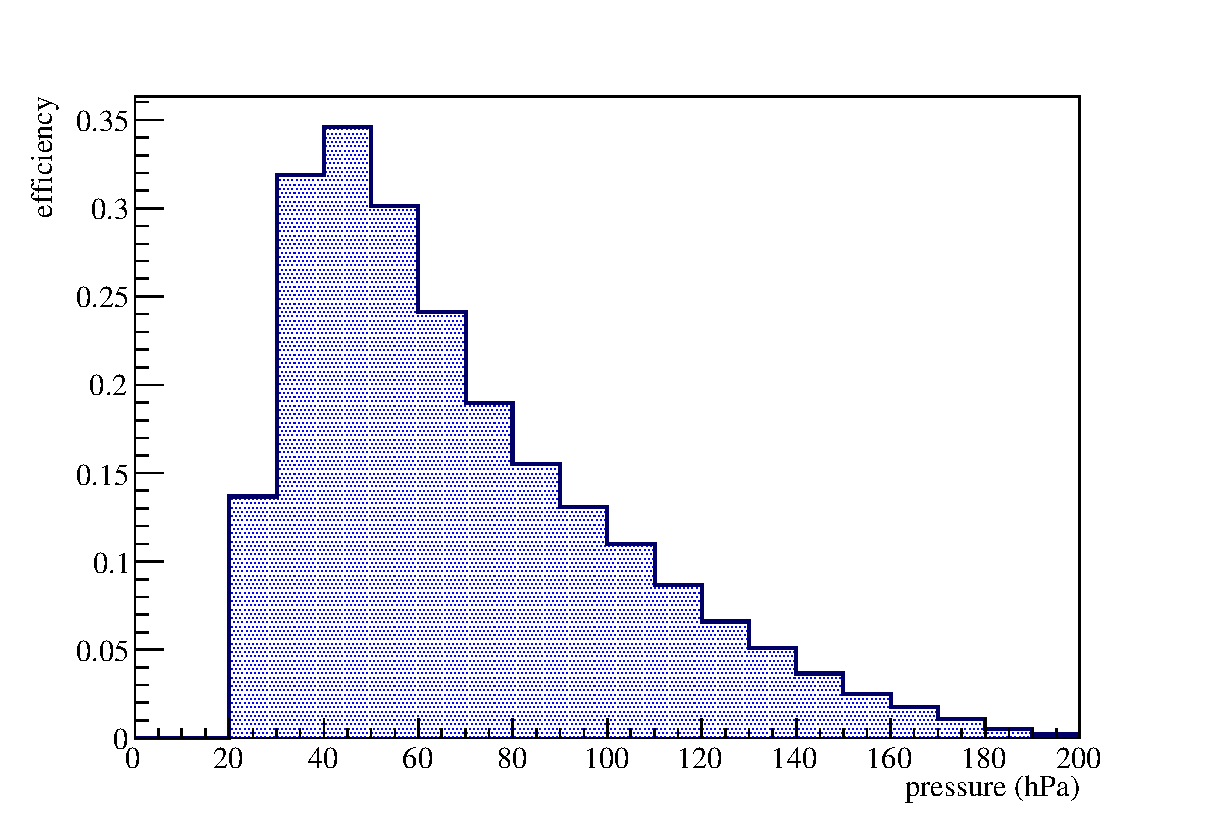
\includegraphics[clip, width=0.7\columnwidth]{eps/efficiency_P_dist.eps}
  \caption[${\rm CH_{4}}$の圧力による検出効率の分布。]
          {${\rm CH_{4}}$の圧力による検出効率の分布。
            $\alpha$粒子は図\ref{fig::alpha_E_dist}に示したエネルギー分布を仮定した。
           }
  \label{fig::efficiency_P_dist}
\end{figure}

50 hPa のときの${\rm CH_{4}}$の各種の値は表\ref{tab::CH4_50_params}のとおりである。
\begin{table}
  \centering
  \caption{50 hPa のときの${\rm CH_{4}}$のパラメータ。}
  \label{tab::CH4_50_params}
  \begin{tabular}{cc}
    \toprule
    項目 & 値\\
    \midrule
    密度 & $3.29\times10^{-5}~{\rm g/cm^{-3}}$\\
    $dE/dx$ ($E_{\alpha} = 0.5~{\rm MeV}$, 10 mm) & 0.107 MeV\\
    飛距離 ($E_{\alpha} = 0.5~{\rm MeV}$) & 65.6 mm\\
    \bottomrule
  \end{tabular}
\end{table}

50 hPa のときの${\rm CH_{4}}$の$dE/dx$と同じ程度になる、他のガスの種類を考えていく。
候補としてiso-${\rm C_{4}H_{10}}$単体と2つの炭化水素に水素とヘリウムの混合ガスの6種類を考える。
単体のガスでは圧力、混合ガスでは圧力を100 hPa に固定し混合比をパラメータとして$dE/dx$を合わせる。
ガスの混合パターン、圧力、$dE/dx$は表\ref{tab::mixture}のとおりである。
分子の括弧は混合の割合を示す。
\begin{table}
  \centering
  \caption[ガスの混合パターン、圧力、$dE/dx$。]
          {ガスの混合パターン、圧力、$dE/dx$。
          括弧はガスの混合の割合を示す。}
  \label{tab::mixture}
  \begin{tabular}{ccccc}
    \toprule
    gas &
    \begin{tabular}{c}
      pressure \\
      (hPa)
    \end{tabular} &
    \begin{tabular}{c}
      density \\
      (${\rm g/cm^{3}}$)
    \end{tabular} &
    \begin{tabular}{c}
      $dE/dx$ (MeV)\\
      $E_{\alpha} = 0.5~{\rm MeV}$ \\
      10 mm
    \end{tabular} &
    \begin{tabular}{c}
      electric field (V/mm) \\
      @ 0.014 mm/ns
    \end{tabular}\\
    \midrule
    ${\rm CH_{4}}$                                & 50  & 3.29$\times 10^{-5}$ & 0.107 & 0.418 \\
    ${\rm CH_{4}} (3) + {\rm H_{2}} (7)$          & 100 & 2.55$\times 10^{-5}$ & 0.107 & 4.31 \\
    ${\rm CH_{4}} (4) + {\rm He} (6)$             & 100 & 3.62$\times 10^{-5}$ & 0.109 & 1.89 \\
%    iso-${\rm C_{4}H_{10}}$                       & 15  & 3.58$\times 10^{-5}$ & 0.102 & 0.644 \\
    iso-${\rm C_{4}H_{10}} (1) + {\rm H_{2}} (9)$ & 100 & 3.13$\times 10^{-5}$ & 0.122 & 6.80 \\
    iso-${\rm C_{4}H_{10}} (1) + {\rm He} (9)$    & 100 & 3.86$\times 10^{-5}$ & 0.102 & 3.26 \\
    \bottomrule
  \end{tabular}
\end{table}
これらの6種類の候補から検出ガスを選ぶ。

\subsection{ドリフトスピード}
MAIKo TPC では100 MHzで1024 samples データを取得するため、ドリフト方向は10.24 $\mu$s のタイムウィンドウが開いている。
ドリフトケージの大きさ ($140\rm{mm}$) を可能な限りタイムウィンドウに収めるためには、
MAIKo TPC のタイムウィンドウ ($10.24\rm{\mu s}$) で140 mmとなるようなドリフトスピード
($140\rm{mm}/10.24\rm{\mu s} \sim 0.014\rm{mm/ns}$) に調整する必要がある。
%($140\rm{mm}/10.24\rm{\mu s} \sim 0.0135\rm{mm/ns}$) に調整する必要がある。

Magboltz~\cite{magboltz} によって計算したドリフト電場とドリフトスピードの関係を図\ref{fig::drift_v_magboltz}に、
ドリフトスピードが0.014 mm/ns となるドリフト電場の値を表\ref{tab::mixture}に示す。
以降、これらのドリフト電場で計算を行う。
\begin{figure}
  \centering
  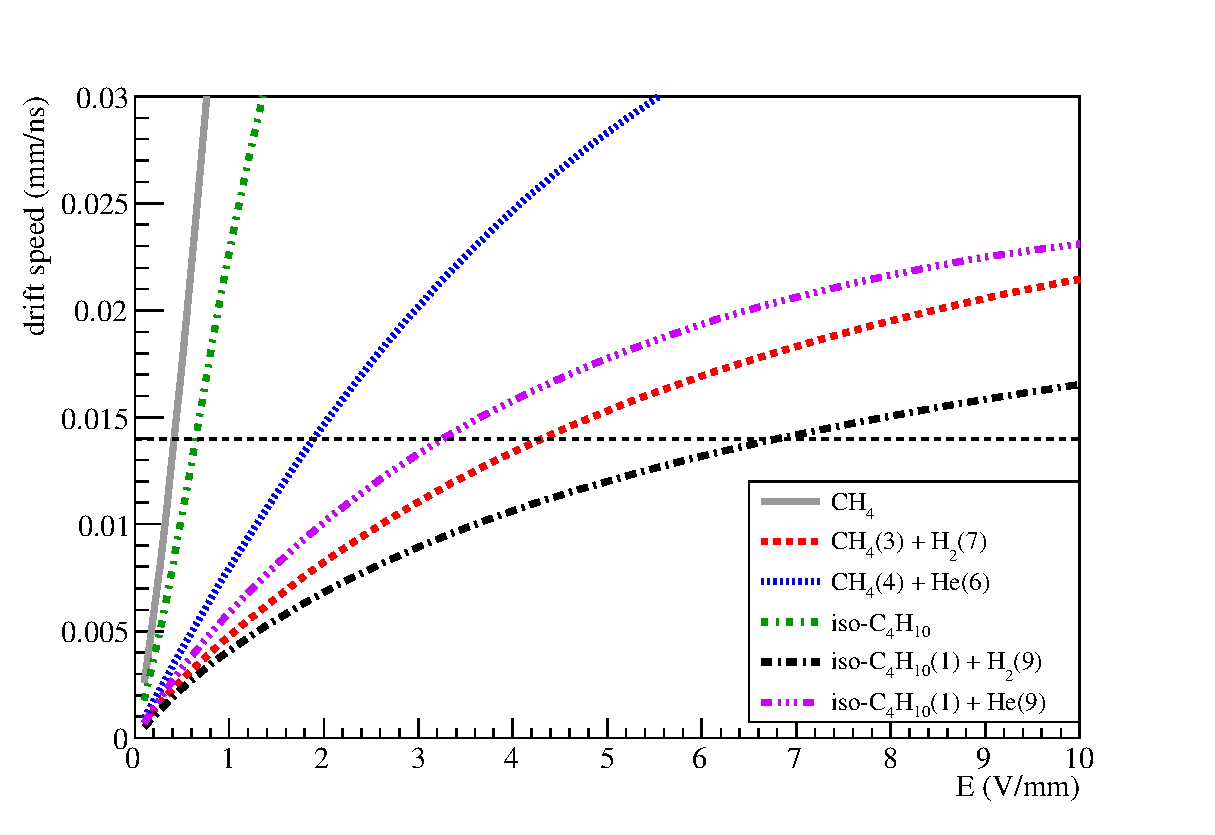
\includegraphics[clip, width=0.9\columnwidth]{eps/drift_v_magboltz.eps}
  \caption[ドリフト電場とドリフトスピードの関係。]
          {ドリフト電場とドリフトスピードの関係。
          ${\rm CH_{4}}$は50 hPa、${\rm C_{4}H_{10}}$は15 hPa、その他は100 hPa である。}
  \label{fig::drift_v_magboltz}
\end{figure}

\subsection{ディフュージョン}
ドリフト電場によって電子が移動する間に検出ガスとの相互作用により拡散 (ディフュージョン) が起きる。
ディフュージョンの効果が大きくなると、$\mu$-PICに到達するまでに荷電粒子で同じ位置に生成された電子が広がるため、
トラックが太く検出される。
トラックが太くなると、複数のトラックを分離するのが難しくなる。
そのため、ディフュージョンの効果が小さいことが望まれる。
Magboltz によって計算したディフュージョンの係数を表\ref{tab::diffusion}に示す。
電子が生成した点から$L$離れた位置で、電子が$\sigma = D\times\sqrt{L}$のガウシアンで広がる。
表\ref{tab::diffusion}中の$D_{t}$は電子の運動方向に対して垂直な方向への拡散、$D_{l}$は電子の運動方向への拡散の係数を表す。
\begin{table}
  \centering
  \caption[Magboltz で計算したディフュージョンの係数。]
          {Magboltz で計算したディフュージョンの係数。
            ディフージョンの大きさはドリフト電場に依存するため、
            ここではドリフトスピードが0.014 mm/ns になるドリフト電場での値を示す。
          $D_{t}$、$D_{l}$はそれぞれ運動方向に垂直、平行方向のディフュージョン。}
  \label{tab::diffusion}
  \begin{tabular}{ccc}
    \toprule
    gas & $D_{t}~(\sqrt{\rm mm})$ & $D_{l}~(\sqrt{\rm mm})$ \\
    \midrule
    ${\rm CH_{4}}$ & 0.433 & 0.547\\
    ${\rm CH_{4} (3) + H_{2} (7)}$ & 0.214 & 0.171\\
    ${\rm CH_{4} (4) + He (6)}$ & 0.270  & 0.248 \\
%    iso-${\rm C_{4}H_{10}}$ & 0.357 & 0.414 \\
    iso-${\rm C_{4}H_{10} (1) + H_{2}}$ & 0.196 & 0.145 \\
    iso-${\rm C_{4}H_{10} (1) + He}$ & 0.246 & 0.197 \\
    \bottomrule
  \end{tabular}
\end{table}
${\rm CH_{4}}$および${\rm C_{4}H_{10}}$の単体ではディフージョンが大きいことが分かる。
同じドリフトスピードのとき、ドリフト電場が大きいほどディフュージョンが小さい。

%\section{$\alpha$線源を用いた測定}
%$\alpha$線源を用いてMAIKo TPC の動作確認を行う。
%線源では、電子のドリフトスピード、増幅率、トラックの太さを確認する。

%\subsection{HV系}
%%ここでは電圧の変数名を説明する。
%
%\subsection{ガス系}
%
%\subsection{回路系}
%
\section{ドリフトスピード}
${}^{241}{\rm Am}$ $\alpha$線源を用いてドリフトスピードの測定を行った。

\subsection{各検出ガスにおけるドリフトスピード}
電子のドリフトスピードを線源によって得られるトラックから求める。
図\ref{pic::collimator}のような線源のコリメータを用いる。
このコリメータはアクリルで作られており、1つの0${}^{\circ}$、4つの30${}^{\circ}$の穴が開いている。
\begin{figure}
  \centering
  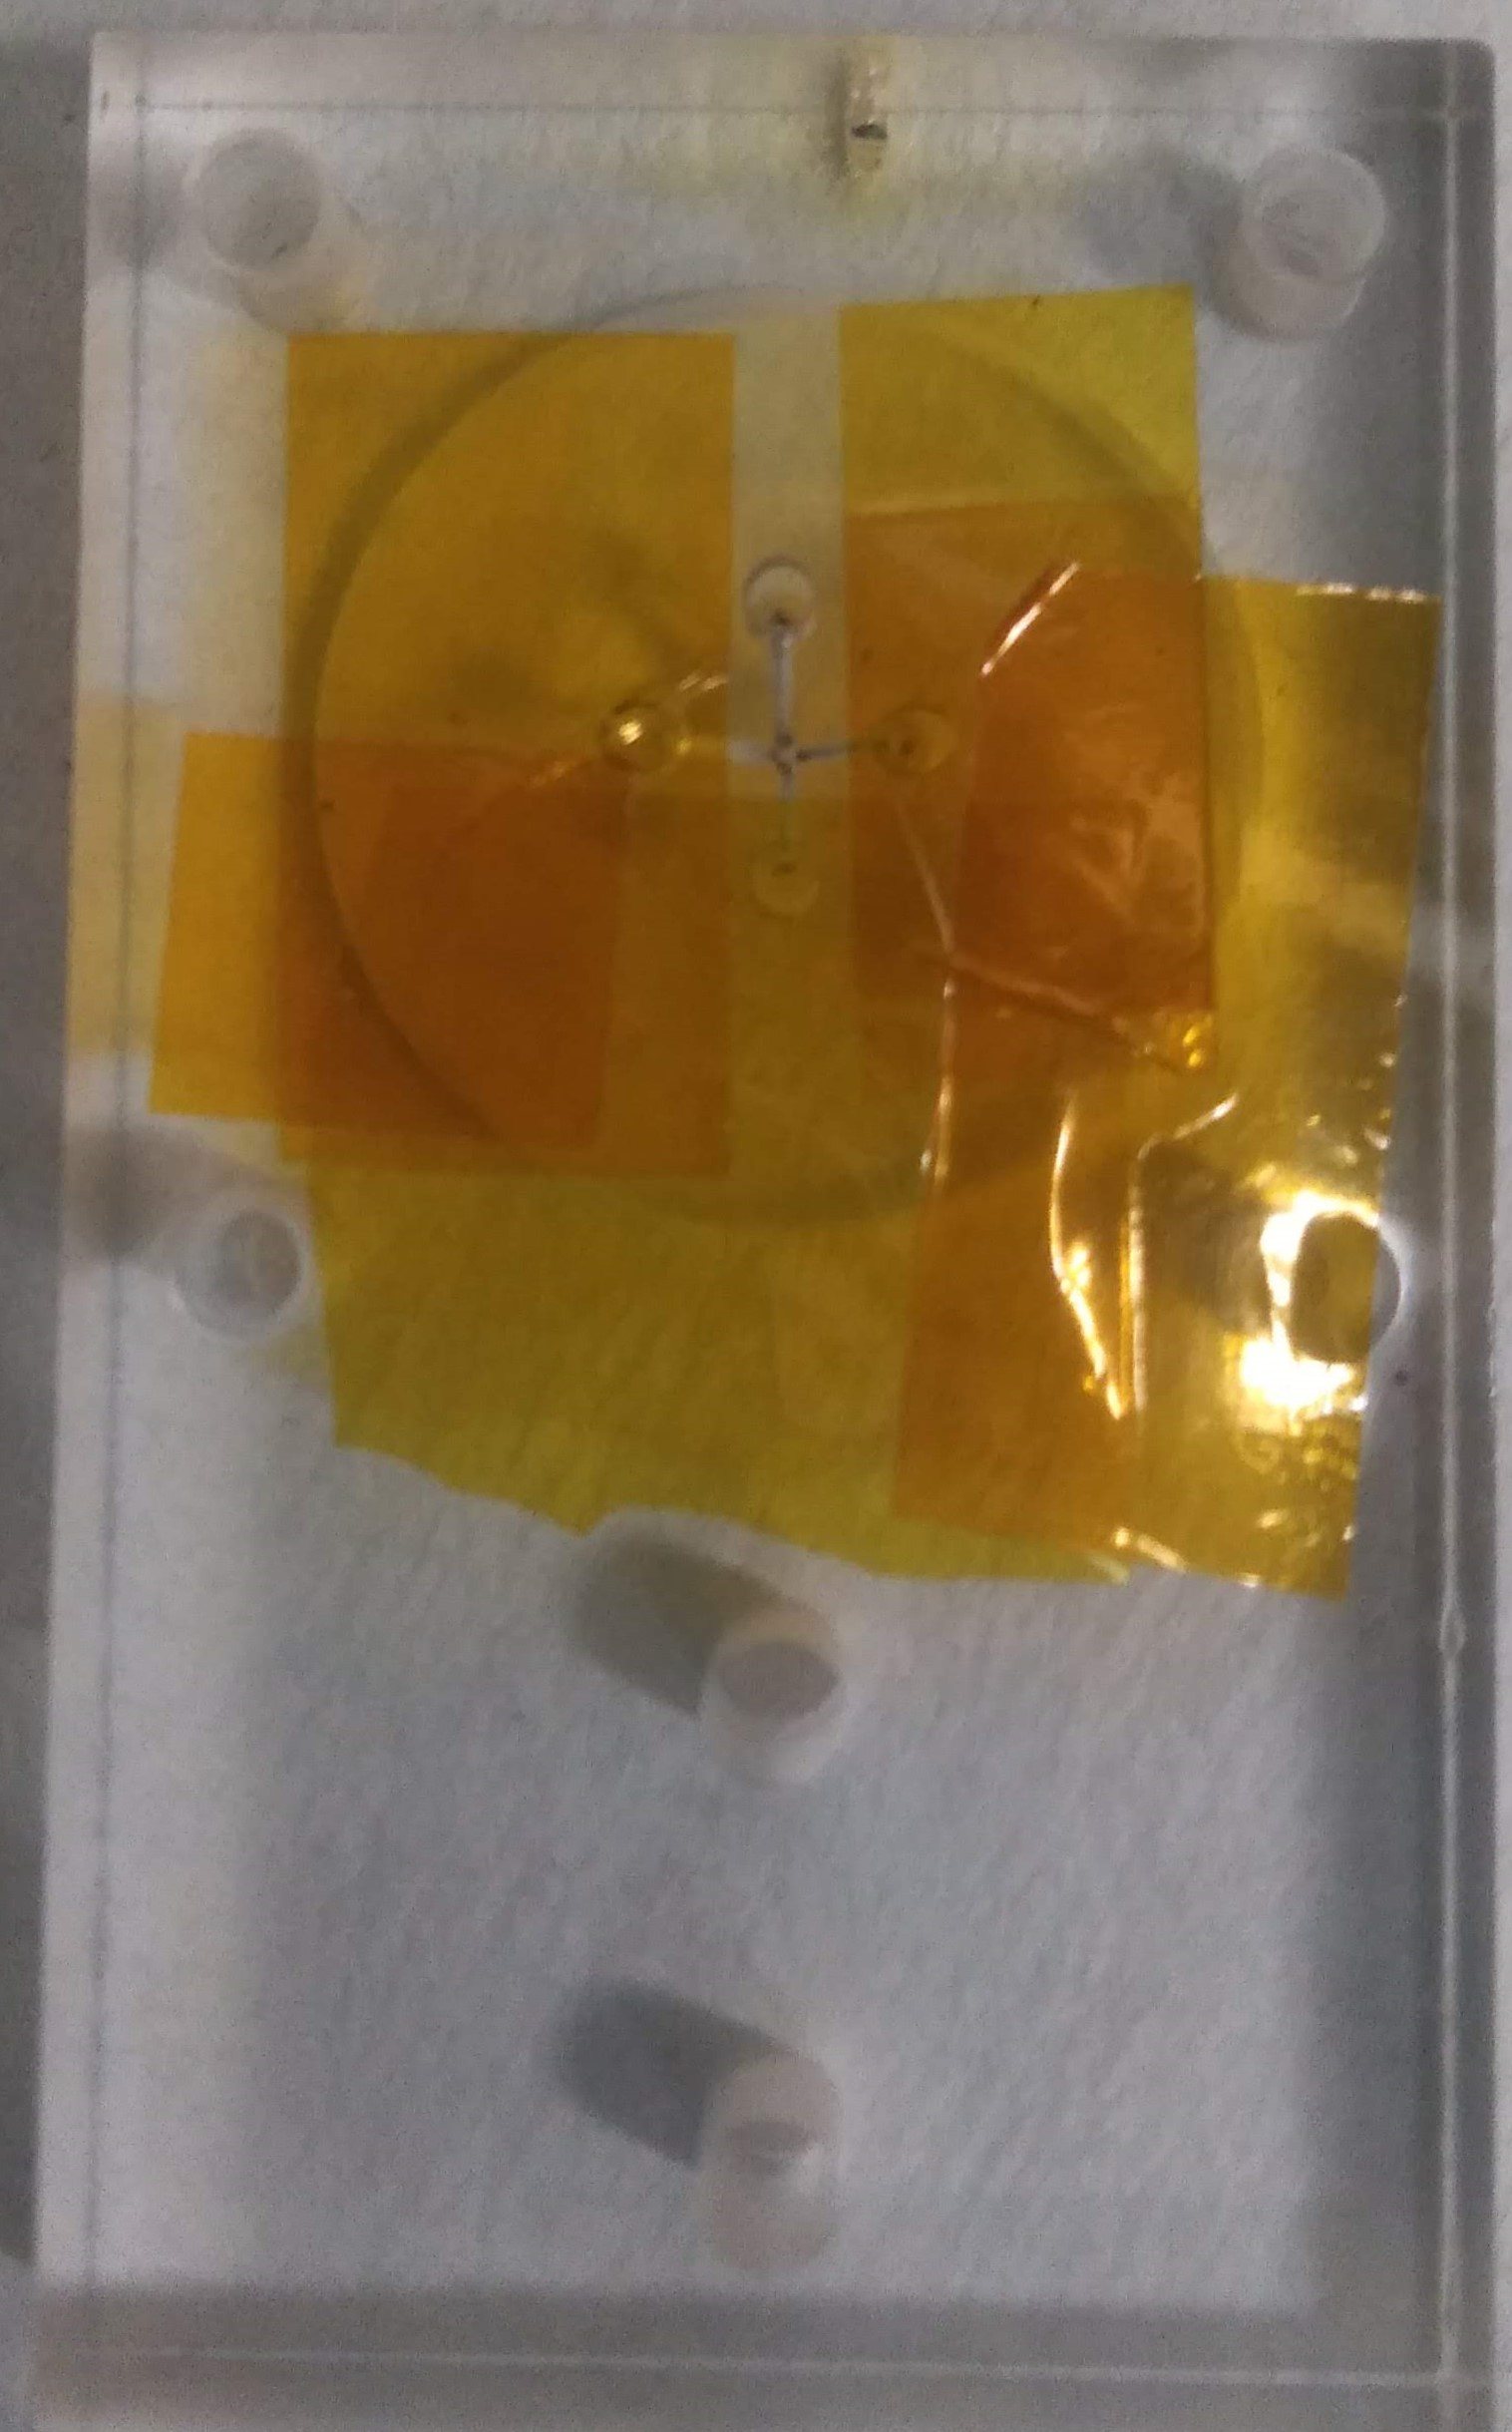
\includegraphics[clip, height=0.7\columnwidth, angle=90]{pic/IMG_20191023_145443_trmd.jpg}
  \caption[線源コリメータ。]
          {線源コリメータ。中央に0${}^{\circ}$、上下左右に30${}^{\circ}$の穴が開いている。}
  \label{pic::collimator}  
\end{figure}
このコリメータを用いることで$\alpha$線を30${}^{\circ}$の方向に限定することができる。
\begin{figure}
  \centering
  \begin{minipage}{0.45\columnwidth}
    \centering
    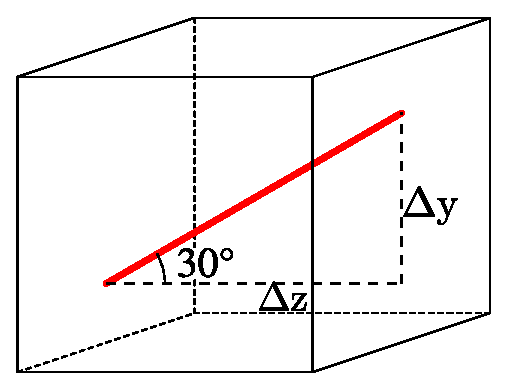
\includegraphics[clip, width=0.9\columnwidth]{eps/drift_v_source.eps}
  \end{minipage}
  \begin{minipage}{0.45\columnwidth}
    \centering
    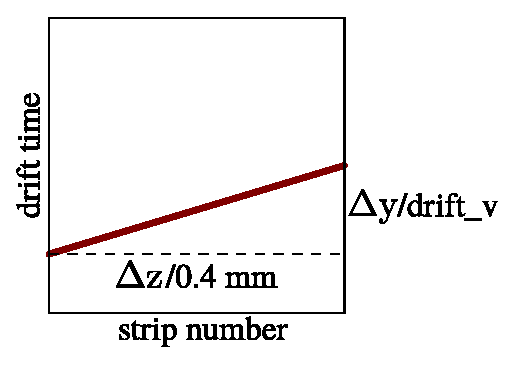
\includegraphics[clip, width=0.9\columnwidth]{eps/drift_v_image.eps}
  \end{minipage}
  \caption[30${}^{\circ}$に方向を限定した$\alpha$線と取得される画像データのイメージ。]
          {30${}^{\circ}$に方向を限定した$\alpha$線 (左) と取得される画像データ (右) のイメージ。}
  \label{fig::drift_v_image}
\end{figure}
図\ref{fig::drift_v_image}の右のようにドリフト方向に$\Delta y$、それと垂直な方向に$\Delta z$移動するとき、
\begin{equation}
  \Delta y = \tan(30^{\circ})\Delta z \label{eq::deltay_deltaz}
\end{equation}
となる。
取得されたデータのトラックが横方向に$\Delta strip$、縦方向に$\Delta t$、
ドリフトスピードを$drift\_v$とすると、
\begin{align}
  \frac{\Delta z}{0.4 {\rm mm}} & = \Delta strip \label{eq::deltaz}\\
  \frac{\Delta y}{drift\_v} & = \Delta t \label{eq::deltay}
\end{align}
式 (\ref{eq::deltay_deltaz}, \ref{eq::deltaz}, \ref{eq::deltay}) より
\begin{equation}
  drift\_v = \frac{\tan(30^{\circ})~\Delta strip\times0.4~{\rm mm}}{\Delta t}
\end{equation}
とドリフトスピードが求まる。

$\alpha$線源を用いて測定したドリフトスピードとMagboltz との比較を
図\ref{fig::drift_v_CH4}, \ref{fig::drift_v_CH4_H2}, \ref{fig::drift_v_CH4_He},
\ref{fig::drift_v_iC4H10_H2}, \ref{fig::drift_v_iC4H10_He}に示す。
\begin{figure}
  \centering
  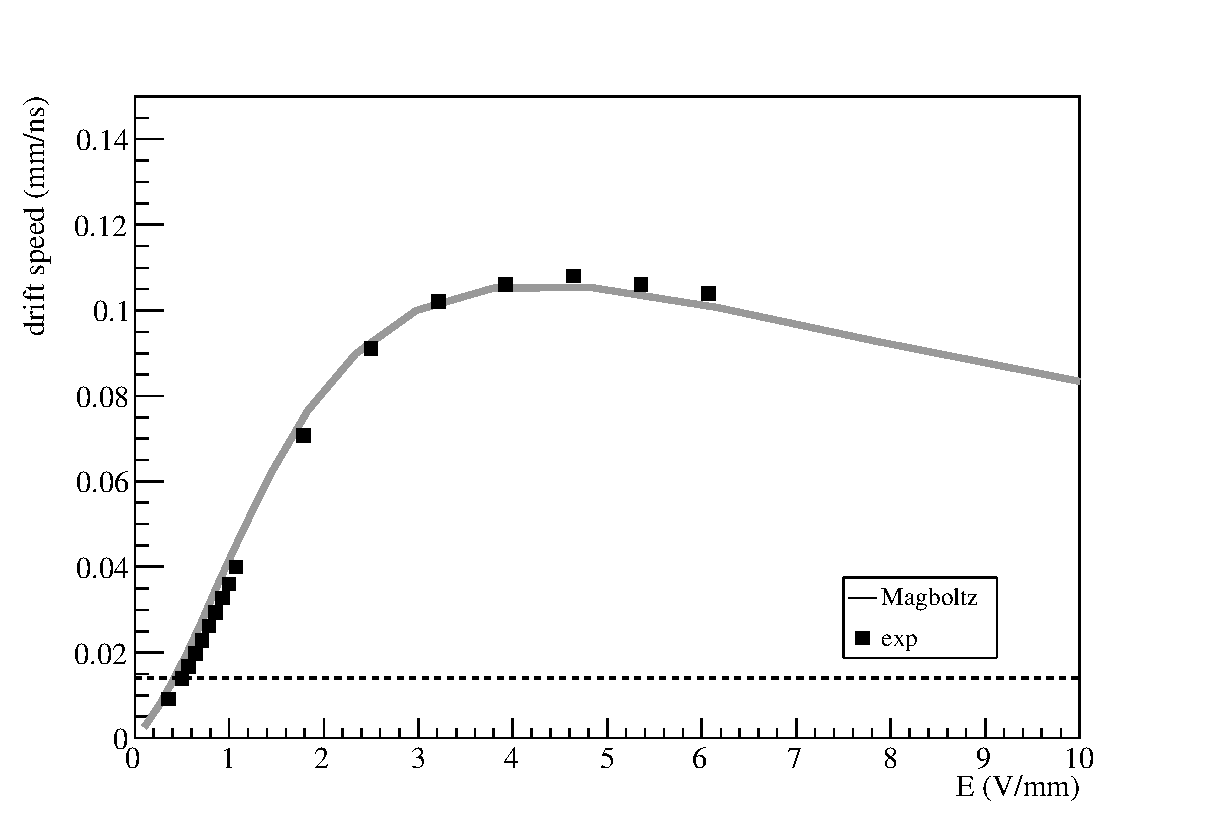
\includegraphics[clip, width=0.9\columnwidth]{eps/drift_v_CH4.eps}
  \caption[検出ガスに${\rm CH_{4}}$を用いたときのドリフトスピードの電場依存性。]
          {検出ガスに${\rm CH_{4}}$を用いたときのドリフトスピードの電場依存性。
            図中の点線は0.014 mm/ns を示す。}
  \label{fig::drift_v_CH4}
%  \includegraphics[clip, width=0.7\columnwidth]{eps/drift_v_CH4_H2.eps}
  \caption{}
  \label{fig::drift_v_CH4_H2}
%  \includegraphics[clip, width=0.7\columnwidth]{eps/drift_v_CH4_He.eps}
  \caption{}
  \label{fig::drift_v_CH4_He}
  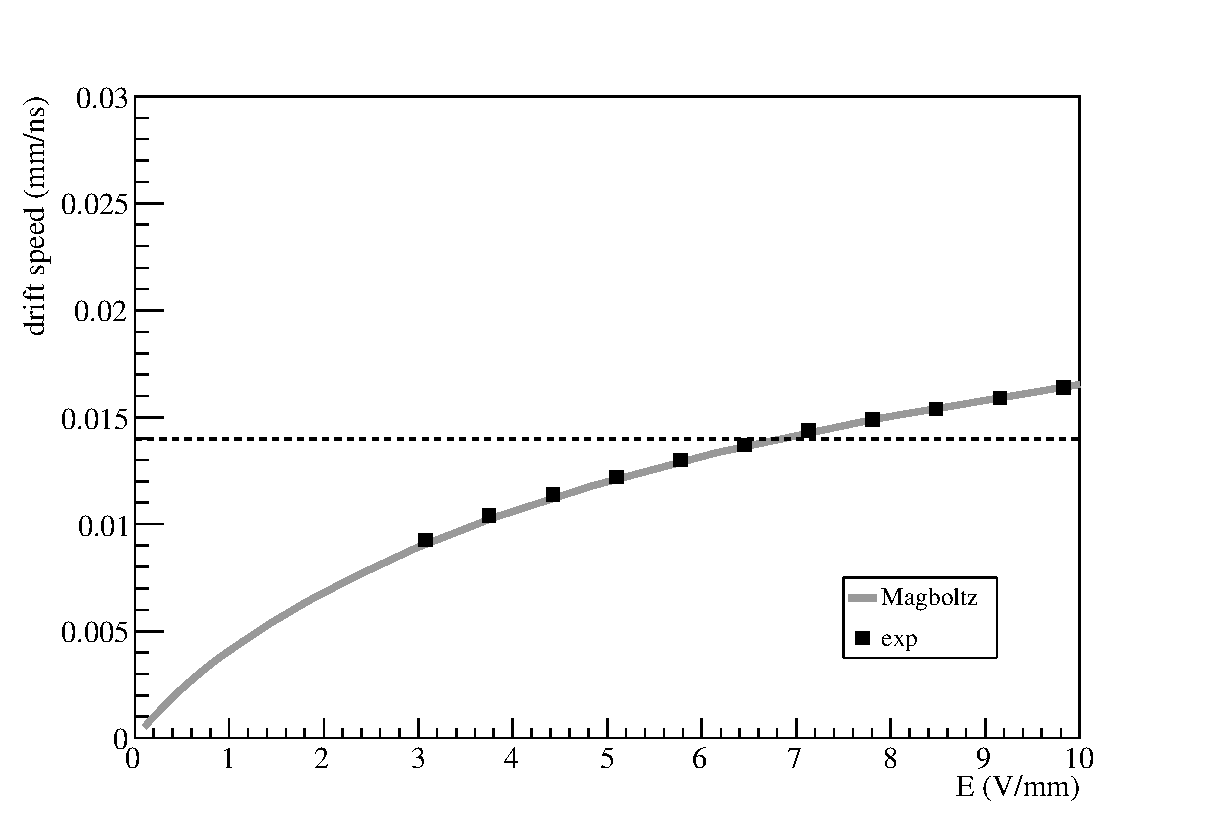
\includegraphics[clip, width=0.9\columnwidth]{eps/drift_v_iC4H10_H2.eps}
  \caption[検出ガスにiso-${\rm C_{4}H_{10}}$を用いたときのドリフトスピードの電場依存性。]
          {検出ガスにiso-${\rm C_{4}H_{10}}$を用いたときのドリフトスピードの電場依存性。
            図中の点線は0.014 mm/ns を示す。}
  \label{fig::drift_v_iC4H10_H2}
%  \includegraphics[clip, width=0.7\columnwidth]{eps/drift_v_iC4H10_He.eps}
  \caption{}
  \label{fig::drift_v_iC4H10_He}
\end{figure}
$\alpha$線源を用いて測定したドリフトスピードと Magboltz を用いて計算したドリフトスピードが一致していることが分かる。

\subsection{ドリフトスピードの時間安定性}
低圧では露点などの不純物が混ざることによって、ドリフトスピードが変化することが懸念される。
そこで、ドリフトスピードの時間安定性の測定を行った。
この測定は$\rm CH_{4}$ 50 hPa で行った。

\section{ガス増幅率}
電圧パラメータを変更させたときの増幅率の変化を測定した。
増幅率を計算するためには荷電粒子が検出ガス中を通過した際に発生する電子数 ($N_{\rm e}$) と
増幅後に$\mu$-PICによって収集された電子数 ($N'_{\rm e}$) の比を取る。
$N_{\rm e}$はガス中での荷電粒子のエネルギー損失とガスのW値から求める。
$N'_{\rm e}$は$\mu$-PICで収集した電荷から求める。
詳しい計算方法について以下で述べる。

ガス中で荷電粒子がエネルギーを落とすと、W値あたり平均1個の電子を電離する。
そのため、荷電粒子のエネルギー損失をW値で割ることで$N_{\rm e}$が求まる。
各ガスのエネルギー損失とW値~\cite{energy_per_ion_pair,pdg}を表\ref{tab::energy_loss_and_W_val}に示す。
測定に用いた$\alpha$線源からは平均4.2 MeVの$\alpha$粒子が出ていることが他の測定によりわかっている。
エネルギー損失は4.2 MeVの$\alpha$粒子が$\mu$-PIC 32 strip分の距離 (12.8 mm) で落とすエネルギーを示している。
\begin{table}
  \centering
  \caption[検出ガスのW値とエネルギー損失と$N_{\rm e}$。]
          {検出ガスのW値とエネルギー損失と$N_{\rm e}$。
          エネルギー損失は荷電粒子がガス中を12.8 mm 進んだ時のものである。}
  \label{tab::energy_loss_and_W_val}
  \begin{tabular}{cccc}
    \toprule
    gas & W (eV) & energy loss (MeV) & $N_{\rm e}$\\
    \midrule
    ${\rm CH_{4}}$                          & 29.1 & 0.0565 & 1.94$\times 10^{3}$ \\
    ${\rm CH_{4} (3) + H_{2} (7)}$          & 34.2 & 0.0534 & 1.56$\times 10^{3}$ \\
    ${\rm CH_{4} (4) + He (7)}$             & 39.2 & 0.0593 & 1.51$\times 10^{3}$ \\
%    iso-${\rm C_{4}H_{10}}$                 & 26.0 & 0.0552 & 2.12$\times 10^{3}$ \\
    iso-${\rm C_{4}H_{10} (1) + H_{2} (9)}$ & 35.4 & 0.0620 & 1.75$\times 10^{3}$ \\
    iso-${\rm C_{4}H_{10} (1) + He (9)}$    & 44.0 & 0.0580 & 1.32$\times 10^{3}$ \\
    \bottomrule
  \end{tabular}
\end{table}

$\mu$-PICからの信号波形は32 strips まとめて図\ref{fig::FADC_waveform}のようなFADC情報として取得している。
この信号波形を時間で積分することによって32 strips で収集した電荷量を計算することができる。
$\mu$-PICで取得した電気信号は読み出し回路内部で800倍に増幅され、
入力インピーダンス50$\Omega$ で電流値を電圧値に変換して取得している。
よって、式 (\ref{eq::N'e})で求めることができる。
$e$は電荷素量である。
\begin{figure}
  \centering
  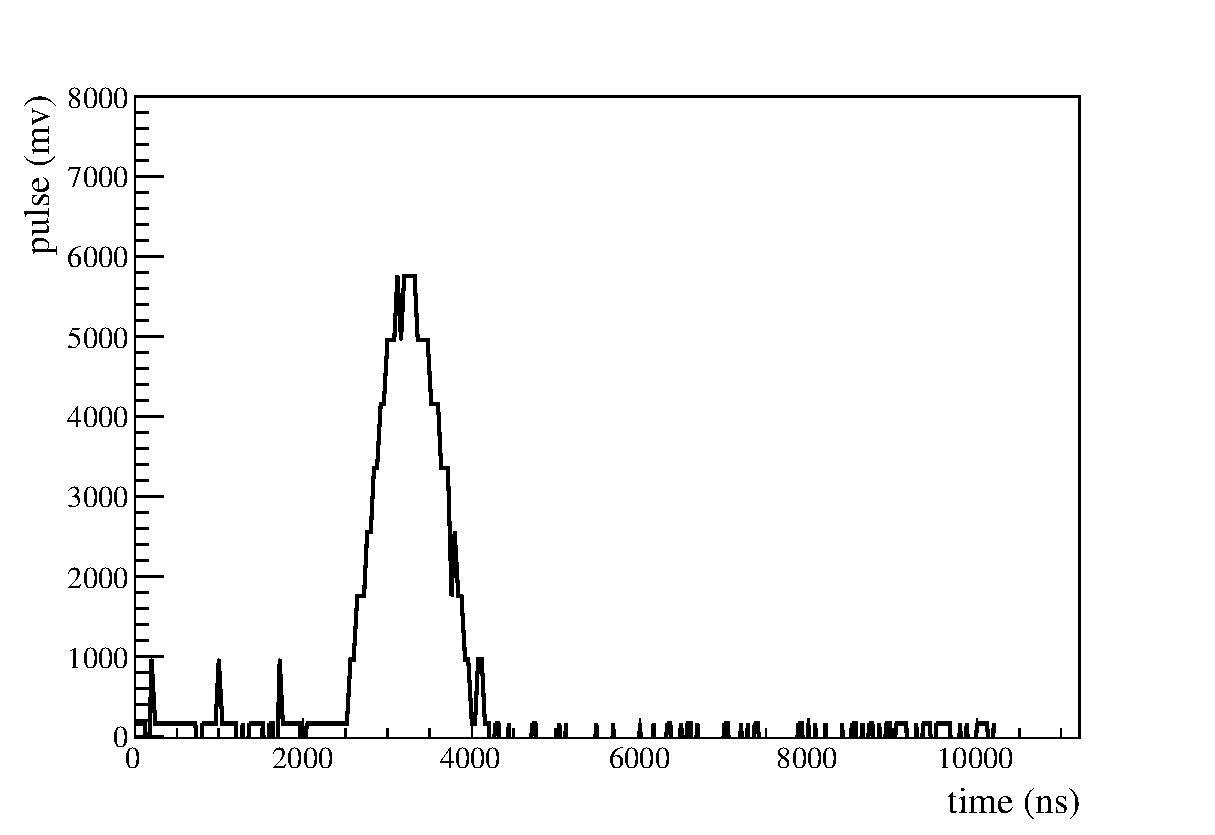
\includegraphics[clip, width=0.7\columnwidth]{eps/0101_waveform_8.eps}
  \caption{FADCで取得された$\mu$-PICの信号波形の一例。}
  \label{fig::FADC_waveform}
\end{figure}
\begin{equation}
  N'_{\rm e} = \frac{\int V (t) dt}{ 50 \times 800 \times e}
  \label{eq::N'e}
\end{equation}

\subsection{GEMによるガス増幅}

\subsection{$\mu$-PICによるガス増幅}

\subsection{GEMとgrid間の電位差による電子の収集効率}

\section{検出ガスの決定}

%ドリフト速度の決定方法は30 degree 方向に$\alpha$線源から$\alpha$を出して、
%その飛跡がデータ上でどう見えるかで決定する。
%ドリフト速度の時間依存性も見た。

%\section{中性子カウンター (液体シンチレータ)}
%\subsection{キャリブレーション}
%\subsection{波形弁別}
%\subsection{検出効率}
%
%\section{中性子カウンター (金属箔)}
%
